\documentclass[12pt,a4paper]{article}
\usepackage[T1]{fontenc}\usepackage[utf8]{inputenc}\usepackage{times}
\usepackage[a4paper,top=2.5cm,bottom=2.5cm,left=2.5cm,right=2.5cm]{geometry}
\usepackage{graphicx}
\graphicspath{{figures/}{figures/dashboard/}}
\usepackage{booktabs}\usepackage{array}\usepackage{enumitem}\usepackage{tabularx}
\usepackage{caption}\usepackage{fancyhdr}\usepackage{parskip}\usepackage{float}
\usepackage{setspace}\onehalfspacing
\usepackage{amsmath}
\usepackage{xurl}\usepackage[hidelinks]{hyperref}
\newcommand{\F}[1]{{\small\url{#1}}}
\captionsetup{font=small,labelfont=bf,labelsep=colon,
              justification=justified,singlelinecheck=false}
\setlist[itemize]{leftmargin=1.3em,itemsep=4pt,topsep=4pt}
\setlist[enumerate]{leftmargin=1.6em,itemsep=6pt,topsep=4pt}
\pagestyle{fancy}\fancyhf{}
\fancyhead[L]{\footnotesize KOUAME Koffi Fid\`ele}
\fancyhead[C]{\footnotesize CUSTOMER ANALYTICS}
\fancyhead[R]{\footnotesize Data Analysis Internship}
\fancyfoot[C]{\thepage}\renewcommand{\headrulewidth}{0.4pt}
\setlength{\headheight}{15pt}

% A dashboard capture: framed with a hairline so a dark screenshot sits cleanly on the page
\newcommand{\capture}[3][\linewidth]{%
\begin{figure}[H]\centering
\setlength{\fboxsep}{0pt}\setlength{\fboxrule}{0.4pt}%
\fbox{\includegraphics[width=\dimexpr#1-0.8pt\relax]{#2}}
\caption{#3}
\end{figure}}

\begin{document}

\begin{titlepage}\centering
\singlespacing
\vspace*{3cm}
{\large\scshape Data Analysis Internship}\\[0.4cm]
{\normalsize Task 9}\\[2.0cm]
\rule{\linewidth}{0.5pt}\\[0.8cm]
{\LARGE\bfseries Customer Analytics}\\[0.6cm]
{\large Data Quality, Measures and Decision Support on 2{,}100 Customers}\\[0.8cm]
\rule{\linewidth}{0.5pt}\\[1.2cm]
{\normalsize Data Cleaning $\bullet$ Measures and KPIs $\bullet$ Statistical Tests
$\bullet$ Insights $\bullet$ Interactive Dashboard $\bullet$ Quality Alerts}\\[3.2cm]
{\large\itshape Prepared by}\\[0.5cm]
{\Large\bfseries KOUAME Koffi Fid\`ele}\\[0.6cm]
{\large 1 October 2026}
\vfill\end{titlepage}

\singlespacing
\tableofcontents\newpage
\onehalfspacing

% =====================================================================
\section{Executive summary}

The brief asks for a complete cleaning, the relevant measures and KPIs, an
interactive dashboard and clear insights, along the chain \emph{raw data, clean
data, measures, insights, decision support}. All are delivered, together with the
notebook that reproduces every number and figure of this report and the pipeline
(ETL, quality gate, scheduling and monitoring) that keeps the dashboard governed.

The extract holds \textbf{2{,}150 rows}. 50 are exact duplicates; once they are
removed, \textbf{2{,}100 customers} remain, each with one purchase made between
27 October 2022 and 23 July 2025.

\textbf{The customers spent \$1{,}021{,}324.} The average ticket is \textbf{\$509.90}
(median \$519.42), computed on the 2{,}003 recorded amounts; 97 amounts (4.6\%) are
missing. The mean satisfaction rating is \textbf{3.03 out of 5}, and 38.7\% of the
valid ratings are 1 or 2.

\textbf{The primary finding concerns the data, not the customers.} Four of the six
quality policies are breached. Only 23.6\% of customers have a usable age: the others
carry the sentinels $-1$ or 200, or nothing. 291 ratings equal 10 on a 1 to 5 scale.
118 purchases carry the impossible date 32/13/2020. 565 purchases (26.9\%) have no
product category, more than any real category. The phone column holds two values for
the whole file and 2{,}100 customers share 144 email addresses: no customer can be
contacted from this register.

\textbf{No customer attribute predicts spending.} The amount does not differ by
category ($p = 0.45$), by gender ($p = 0.10$), with age ($\rho = 0.02$) or with the
rating ($\rho = -0.03$). Amounts are spread evenly between \$5 and \$1{,}000
($p = 0.49$).

\textbf{There is no seasonality.} The dashboard's monthly chart shows a dip in August
and September. It comes from coverage: those two months appear in two years of data,
the others in three. On the 32 complete months, purchases are even ($p = 0.11$).

What the register supports well is the customer count, revenue, the average ticket
and the satisfaction level. Targeting, contact and demographic analysis must wait for
the capture to be repaired.

% =====================================================================
\section{Data and method}

\subsection{The register}

One row is one customer and one purchase. The columns are the customer identifier,
name, email and phone, age and gender, the purchase amount, date and product category
(Books, Clothing, Electronics, Home, Toys), and a satisfaction rating on the 1 to 5
scale. The file also carries two export artefacts: an empty column \F{Unnamed} and an
exact copy of \F{Gender}.

\subsection{Process}

The analysis follows five steps, each implemented as a section of the notebook
\F{Customer-Analytics.ipynb}:

\begin{enumerate}
\item \textbf{Quality audit.} Eight checks, one per defect family: duplicates, export
artefacts, sentinel ages, out-of-scale ratings, the sentinel date, gender spellings
and missing categories, contact fields, and the purchase amount.
\item \textbf{Cleaning.} Certain errors are corrected, uncertain values are flagged,
and only exact duplicate rows are removed. The notebook checks that its cleaning
gives the same table as the production pipeline \F{etl/run_etl.py}.
\item \textbf{Measures.} Each indicator is computed on the population that can
support it, and that population is stated with the value.
\item \textbf{Tests.} Every segment difference is tested before it is reported:
Kruskal--Wallis and Mann--Whitney for amounts across groups, chi-square for mixes
and monthly counts, Spearman rank correlation for associations, Kolmogorov--Smirnov
for the shape of the amount distribution.
\item \textbf{Decision support.} Each finding is translated into an action and an
owner, exposed in an interactive dashboard and guarded by automated quality alerts.
\end{enumerate}

The analysis uses Python only (pandas, NumPy, SciPy, Matplotlib). No spreadsheet
and no business-intelligence tool is used at any stage.

% =====================================================================
\section{Data quality}

\begin{table}[H]\centering\singlespacing
\caption{Checks performed on the register, counted on the 2{,}100 customers after
de-duplication}
\small
\begin{tabular}{@{}lrr@{}}
\toprule
\textbf{Check} & \textbf{Rows} & \textbf{Share} \\ \midrule
Rows as supplied & 2{,}150 & \\
Exact duplicate rows (repeated CustomerID) & 50 & 2.3\% \\
Customers after de-duplication & 2{,}100 & 100\% \\ \midrule
Age missing or sentinel ($-1$, 200) & \textbf{1{,}605} & \textbf{76.4\%} \\
Rating missing & 322 & 15.3\% \\
Rating out of scale (10) & 291 & 13.9\% \\
Product category missing & \textbf{565} & \textbf{26.9\%} \\
Gender missing & 267 & 12.7\% \\
Purchase date invalid (32/13/2020) & \textbf{118} & \textbf{5.6\%} \\
Purchase amount missing & 97 & 4.6\% \\
Phone missing or placeholder & 2{,}100 & 100\% \\
\bottomrule
\end{tabular}
\end{table}

\subsection{The defects are sentinels, not typing errors}

Every defect of the file is a repeated default value. The 1{,}099 invalid ages are
two values only, $-1$ (553) and 200 (546). The 291 out-of-scale ratings are all 10.
The 118 invalid dates are all the same string, 32/13/2020. The phone column holds
two numbers, 123456789 and 987654321, and is empty elsewhere. A defect repeated
hundreds of times is a system default written when the real value was not captured;
the fix therefore belongs to the capture forms, not to the analysis.

\begin{figure}[H]\centering
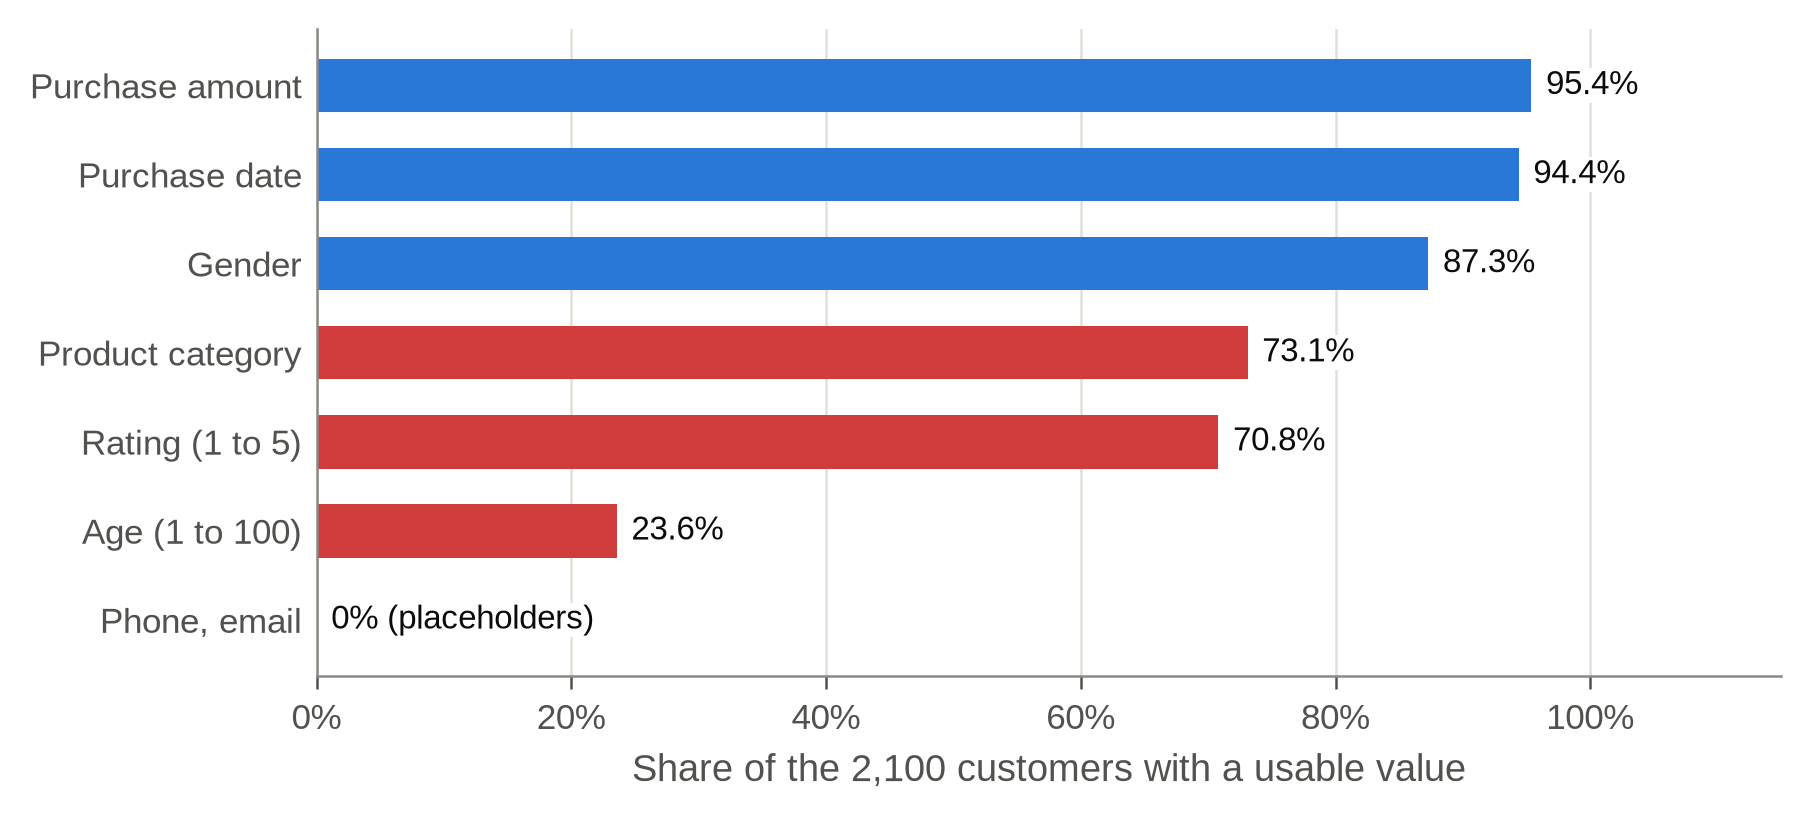
\includegraphics[width=\linewidth]{01_data_quality.png}
\caption{Share of the 2{,}100 customers with a usable value in each analytical
column after cleaning. Columns below 80\% are shown in red. Amount, date and gender
are usable; category, rating and above all age are not complete enough for segment
analysis, and the contact fields are placeholders.}
\end{figure}

\begin{figure}[H]\centering
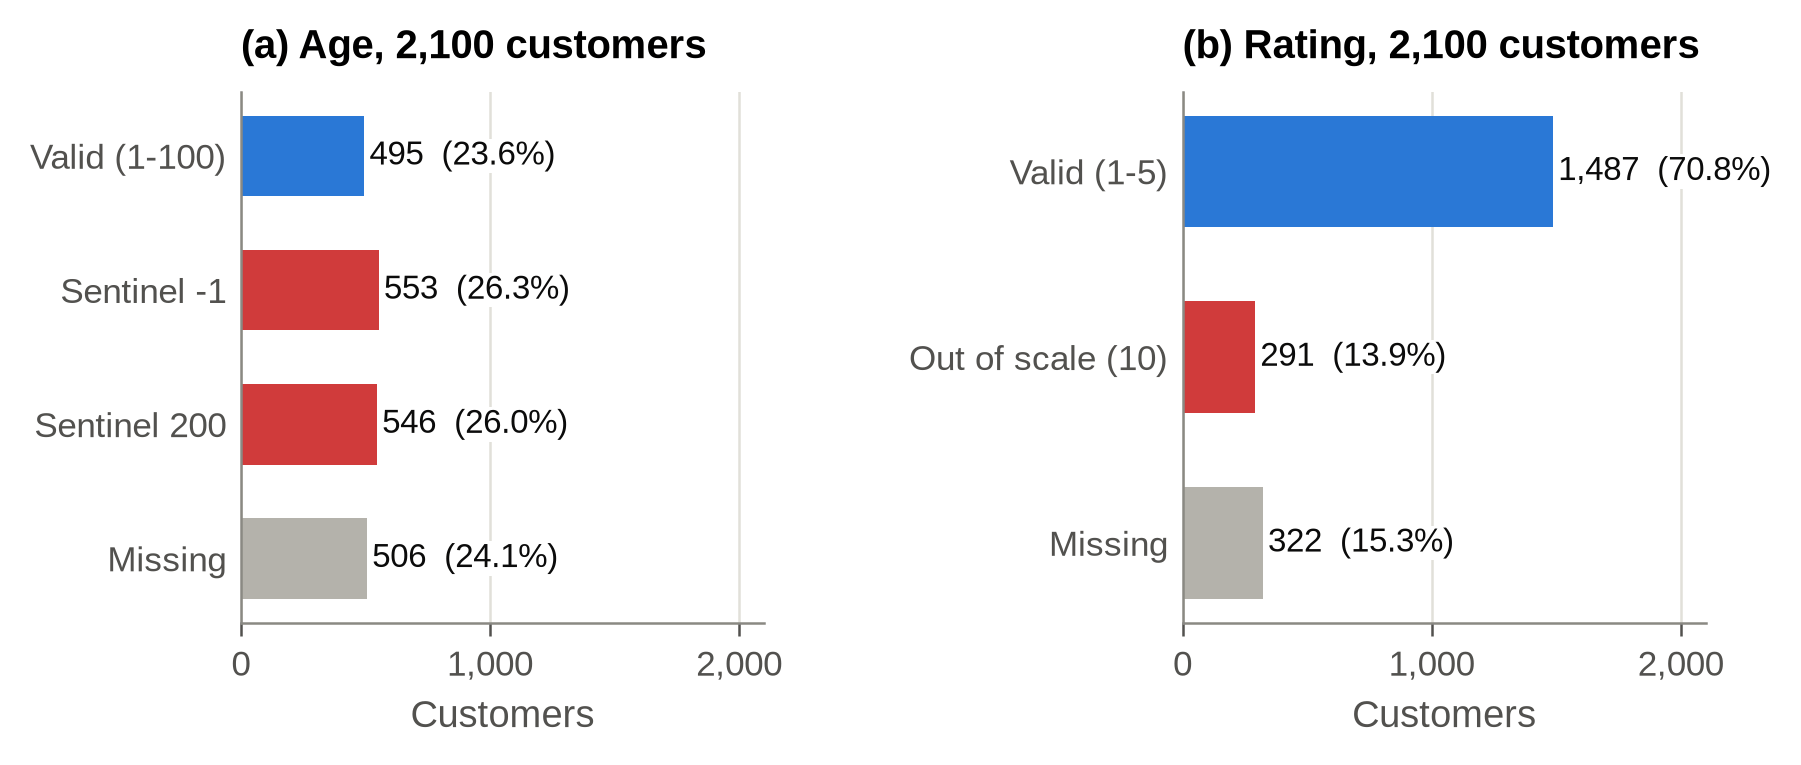
\includegraphics[width=\linewidth]{02_age_rating_raw.png}
\caption{What the raw age (a) and rating (b) columns contain. The two age sentinels
weigh as much as the valid ages and the missing values together; a mean on the raw
column gives 85 years instead of 54.4. The 10s raise the raw mean rating from 3.03
to 4.17.}
\end{figure}

% =====================================================================
\section{Cleaning}

\begin{table}[H]\centering\singlespacing
\caption{One decision per problem, with the reason for it}
\small
\begin{tabularx}{\linewidth}{@{}p{3.3cm}r X@{}}
\toprule
\textbf{Problem} & \textbf{Count} & \textbf{Decision and reason} \\ \midrule
Duplicate CustomerID & 50 & First row kept. Each duplicate is an exact copy of its
first row, field by field, so no information is lost. \\
Export artefacts & 2 columns & \F{Unnamed} (empty) and the copy of \F{Gender}
dropped. \\
Gender spellings & 1{,}833 & Six spellings (M, male, Male, F, female, Female)
mapped to Male and Female; 267 left missing. \\
Sentinel ages & 1{,}099 & Set to missing, not to a mean. An imputed age would invent
a demographic profile for three customers in four. \\
Ratings of 10 & 291 & Set to missing. They could be 1 or 5 on a reversed scale;
neither can be proved. \\
Sentinel date & 118 & Flag \F{DateInvalid}, date left empty. The purchase, amount
and rating remain usable. \\
Missing category & 565 & Labelled \F{Unknown} and kept, so that revenue totals
remain complete. \\
Missing amount & 97 & Flag \F{AmountMissing}, kept missing. \\
\bottomrule
\end{tabularx}
\end{table}

Every flagged row is kept, so a reader can include or exclude it and see the
difference. The clean file \F{data/customers_clean.csv} has 2{,}100 rows. The
notebook's cleaning and the production pipeline \F{etl/run_etl.py} produce the same
table, column by column.

% =====================================================================
\section{Indicators}

\begin{table}[H]\centering\singlespacing
\caption{Each indicator with the population it is computed on}
\small
\begin{tabular}{@{}lrl@{}}
\toprule
\textbf{Indicator} & \textbf{Value} & \textbf{Computed on} \\ \midrule
Customers & 2{,}100 & distinct CustomerID \\
Revenue & \$1{,}021{,}324 & 2{,}003 recorded amounts \\
Average ticket & \$509.90 & 2{,}003 recorded amounts \\
Median ticket & \$519.42 & 2{,}003 recorded amounts \\ \midrule
Mean rating & 3.03 / 5 & 1{,}487 valid ratings \\
Ratings of 1 or 2 & 38.7\% & 1{,}487 valid ratings \\ \midrule
Male / female & 51.4\% / 48.6\% & 1{,}833 known genders \\
Mean age & 54.4 years & 495 valid ages \\ \midrule
Unknown category & 565 (26.9\%) & all customers \\
Invalid dates & 118 (5.6\%) & all customers \\
Missing amounts & 97 (4.6\%) & all customers \\
\bottomrule
\end{tabular}
\end{table}

Most indicators name their own base. Revenue rests on 2{,}003 amounts, the rating on
1{,}487 and the mean age on 495. Writing the base beside the number is better than a
footnote, because a footnote does not travel when a figure is copied into a slide.

% =====================================================================
\section{Results}

\subsection{What is bought}

\begin{figure}[H]\centering
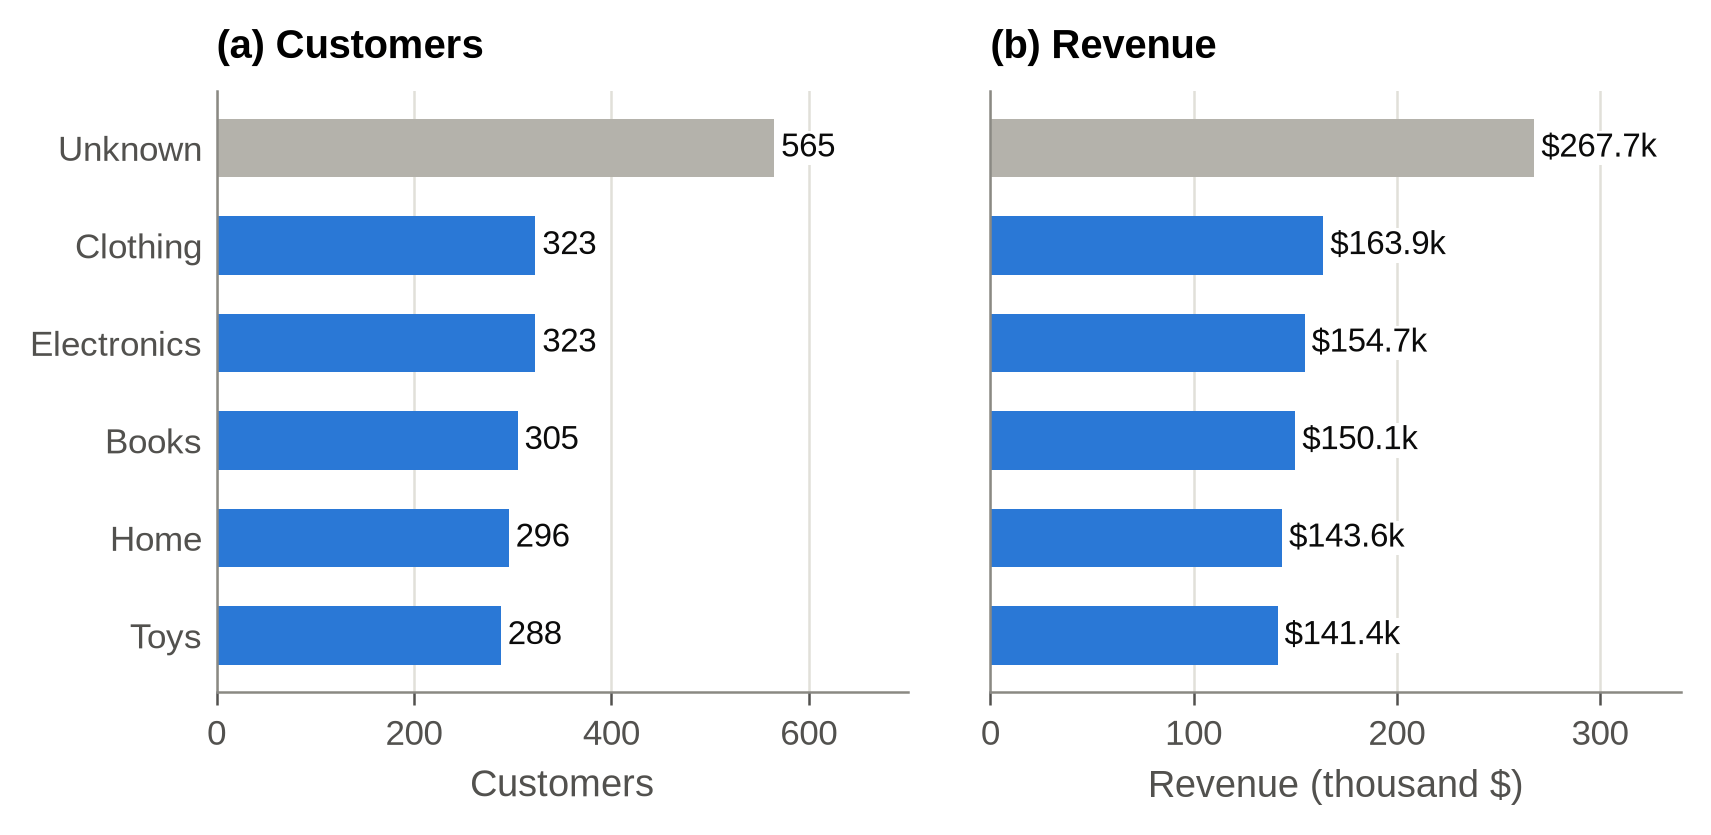
\includegraphics[width=\linewidth]{03_categories.png}
\caption{Customers (a) and revenue (b) by product category, in the same order.
\emph{Unknown} (grey) is a capture gap, larger than any real category. Among the five
categories, Clothing leads revenue (\$163{,}865) and Toys trails (\$141{,}384), a
gap of 14\%.}
\end{figure}

The five real categories are close in size, from 288 (Toys) to 323 customers
(Clothing and Electronics, tied). Because the \emph{Unknown} purchases do not differ
from the others in amount ($p = 0.21$), the shares of the known categories are a fair
guide to the mix, but every category total is understated by about a quarter.

\begin{figure}[H]\centering
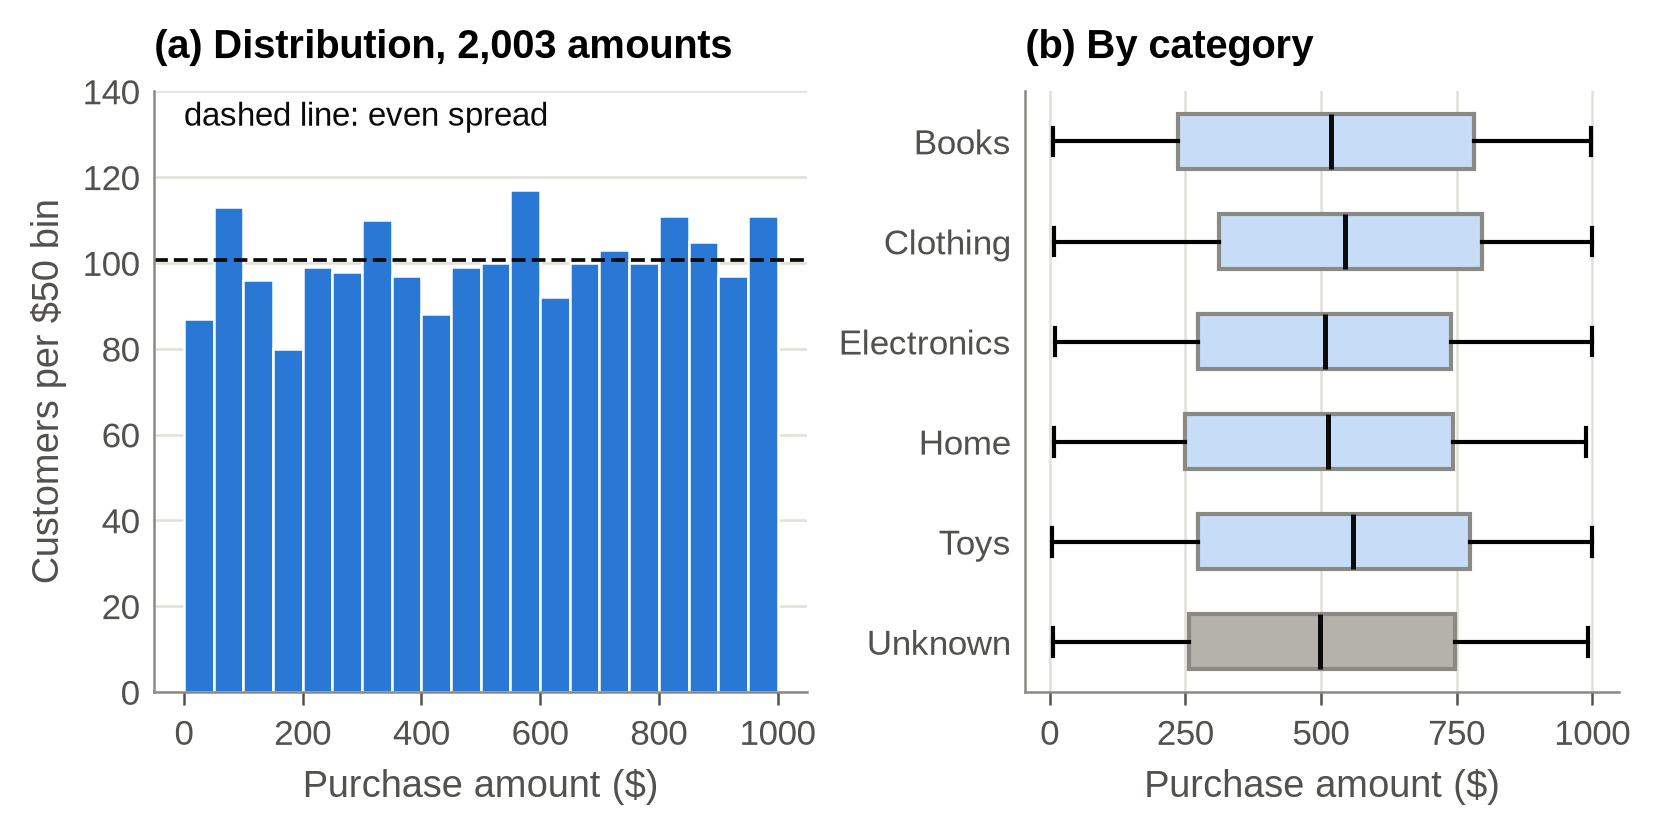
\includegraphics[width=\linewidth]{04_amounts.png}
\caption{Distribution of the 2{,}003 recorded amounts in bins of \$50, against the
count expected if amounts were spread evenly (dashed line) (a), and amounts by
category (b). Boxes show the interquartile range and black lines the median. The
distribution is flat from \$5 to \$1{,}000 (Kolmogorov--Smirnov $p = 0.49$), and the
categories do not differ (Kruskal--Wallis $p = 0.45$).}
\end{figure}

\subsection{Purchases through time}

\begin{figure}[H]\centering
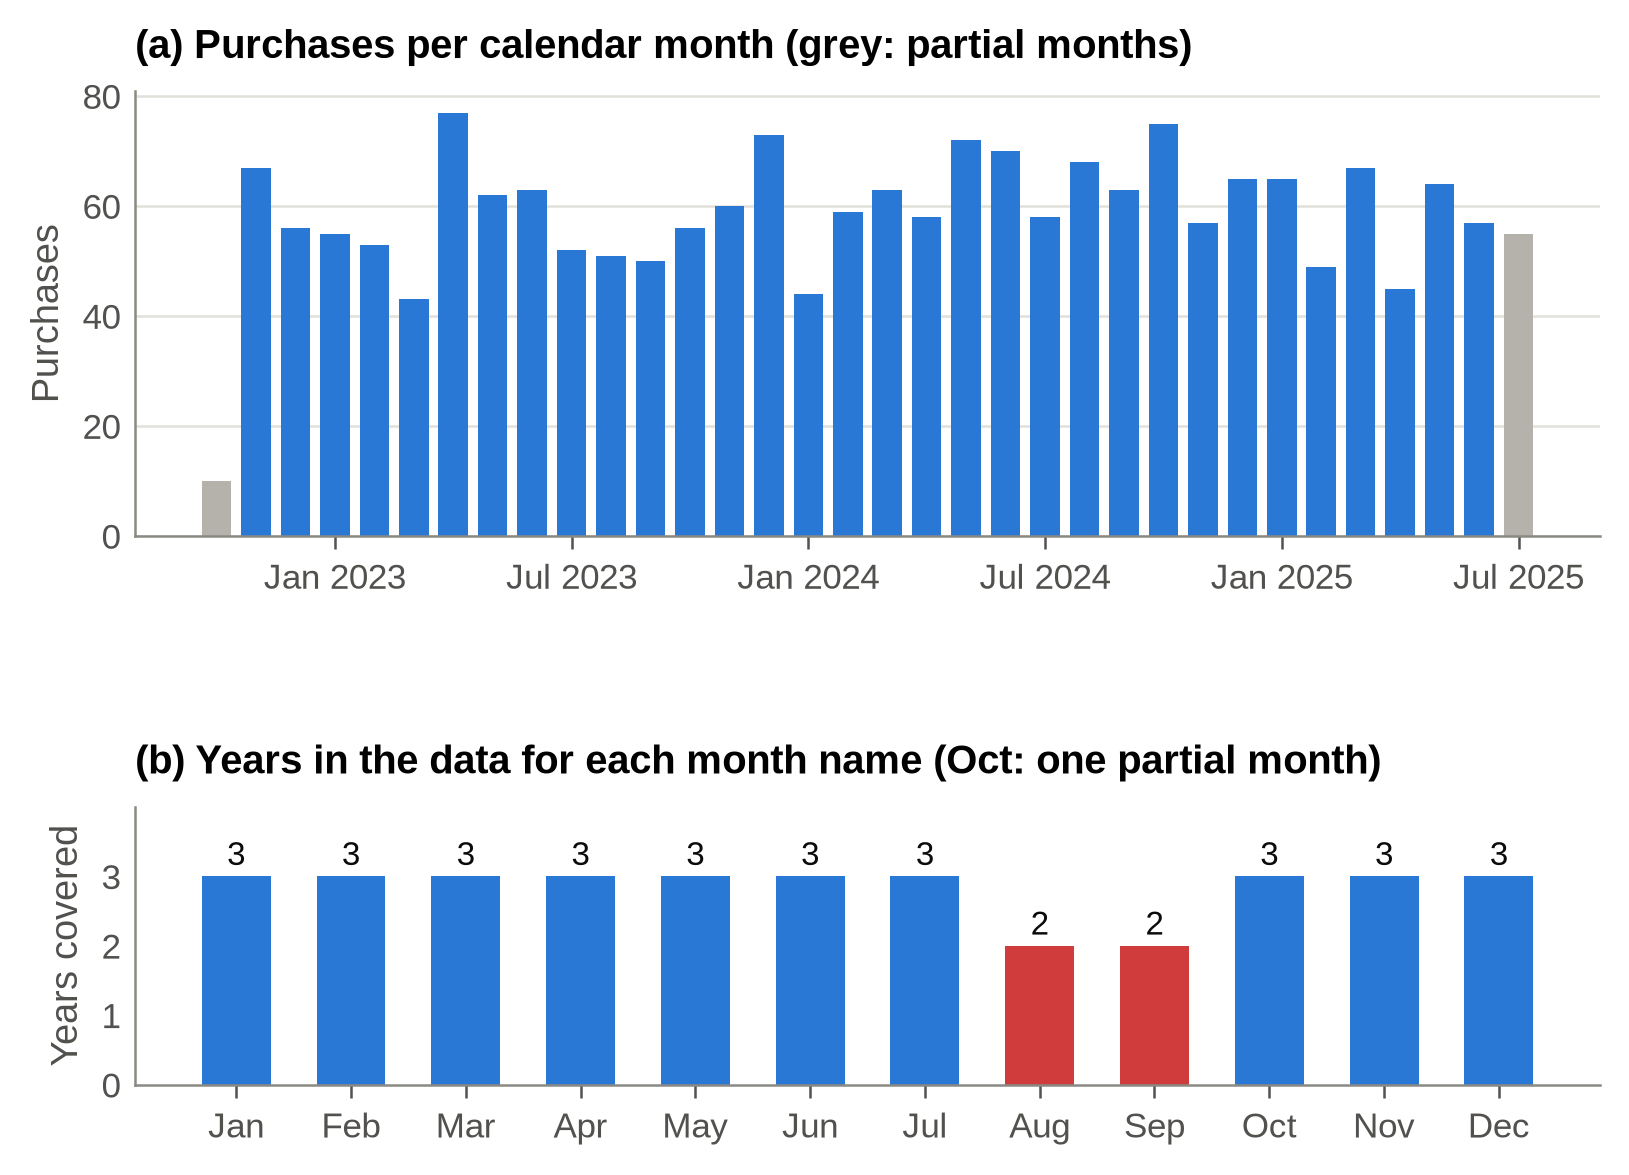
\includegraphics[width=\linewidth]{05_monthly.png}
\caption{Purchases per calendar month from October 2022 to July 2025 (a); the first
and last months are partial (grey). Number of years present in the data for each
month name (b). August and September appear in two years, every other month in three.
On the 32 complete months, purchases are compatible with an even spread (chi-square
$p = 0.11$).}
\end{figure}

\begin{table}[H]\centering\singlespacing
\caption{The pooled monthly count divided by the number of years covered}\label{tab:pooled}
\small
\begin{tabular}{@{}lrrrrrrrrrrrr@{}}
\toprule
 & Jan & Feb & Mar & Apr & May & Jun & Jul & Aug & Sep & Oct & Nov & Dec \\ \midrule
Pooled count & 164 & 161 & 173 & 180 & 198 & 190 & 165 & 119 & 113 & 141 & 184 & 194 \\
Years covered & 3 & 3 & 3 & 3 & 3 & 3 & 3 & 2 & 2 & 3 & 3 & 3 \\
Per year & 54.7 & 53.7 & 57.7 & 60.0 & 66.0 & 63.3 & 55.0 & 59.5 & 56.5 & 47.0 & 61.3 & 64.7 \\
\bottomrule
\end{tabular}
\end{table}

Once divided by the years covered, August and September sit in the middle of the
range. October is the lowest only because October 2022 holds the first five days of
the period (10 purchases).

\subsection{Who the customers are}

\begin{figure}[H]\centering
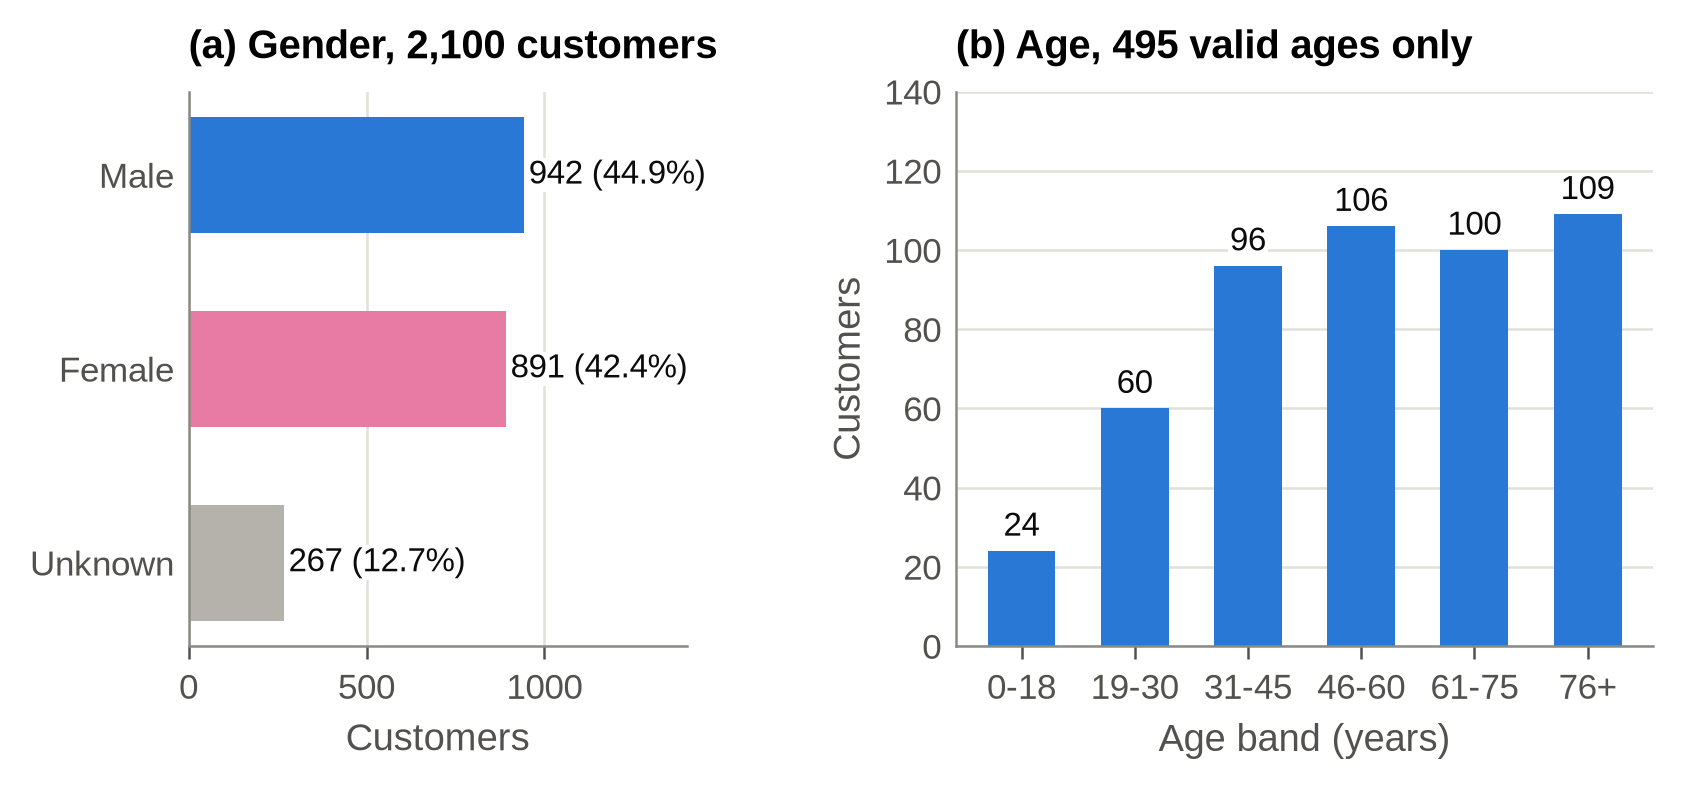
\includegraphics[width=\linewidth]{06_demographics.png}
\caption{Gender of the 2{,}100 customers (a) and age bands of the 495 customers with
a valid age (b). Where gender is known, the split is 51.4\% male and 48.6\% female.
The age bands describe 23.6\% of customers only and cannot be generalised.}
\end{figure}

Men and women do not differ in spending (Mann--Whitney $p = 0.10$): average ticket
\$499 for men, \$522 for women.

\subsection{Satisfaction}

\begin{figure}[H]\centering
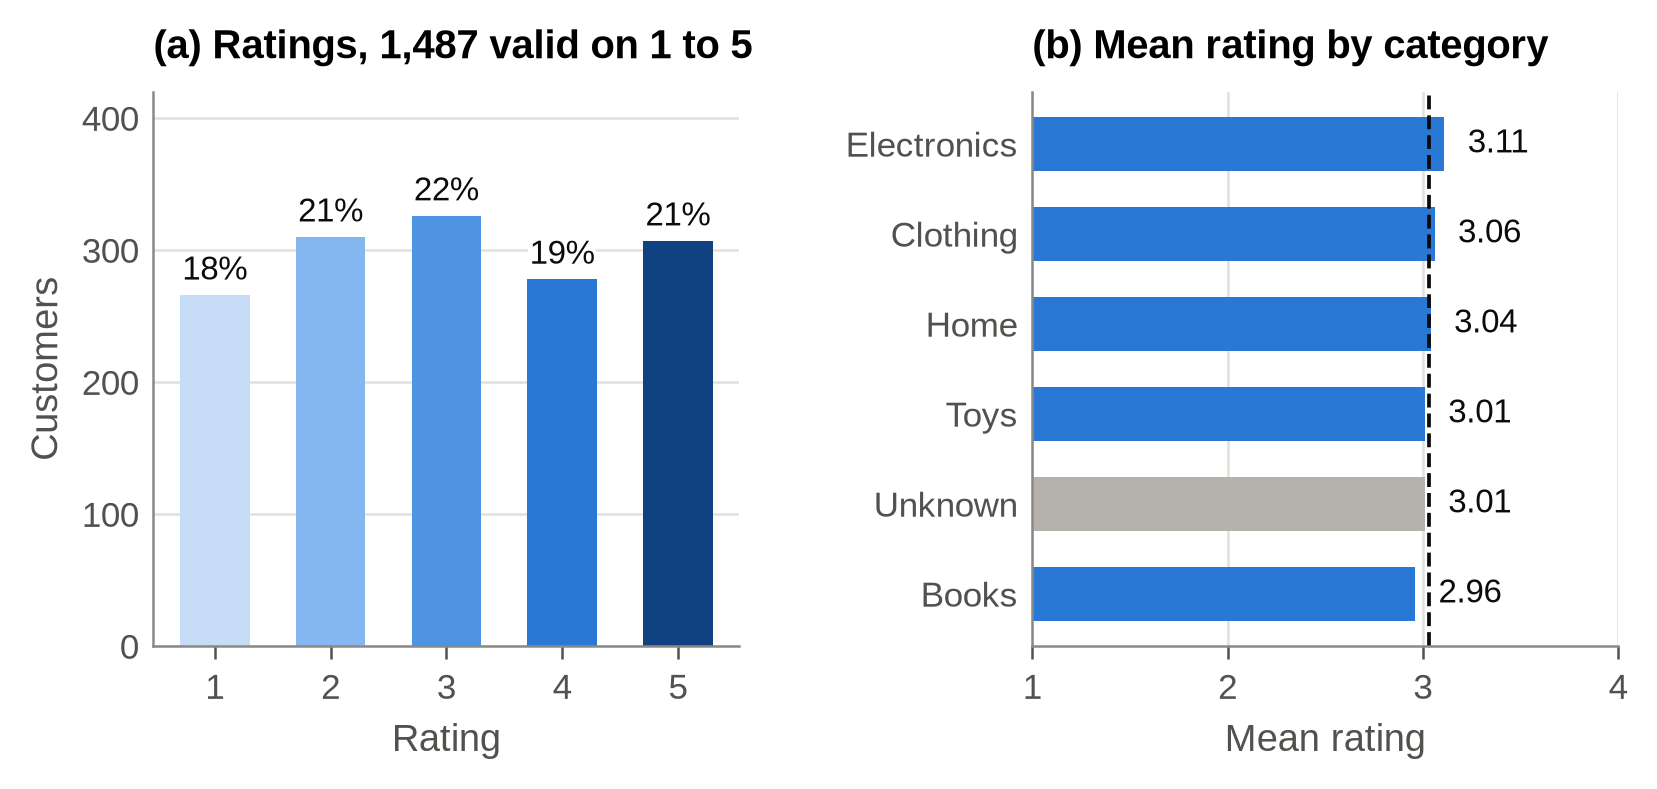
\includegraphics[width=\linewidth]{07_ratings.png}
\caption{Distribution of the 1{,}487 valid ratings (a) and mean rating by category
against the overall mean of 3.03 (dashed line) (b). The five scores are almost equally
frequent (18\% to 22\%), and the rating mix does not depend on the category
(chi-square $p = 0.94$).}
\end{figure}

\subsection{What drives the amount}

\begin{figure}[H]\centering
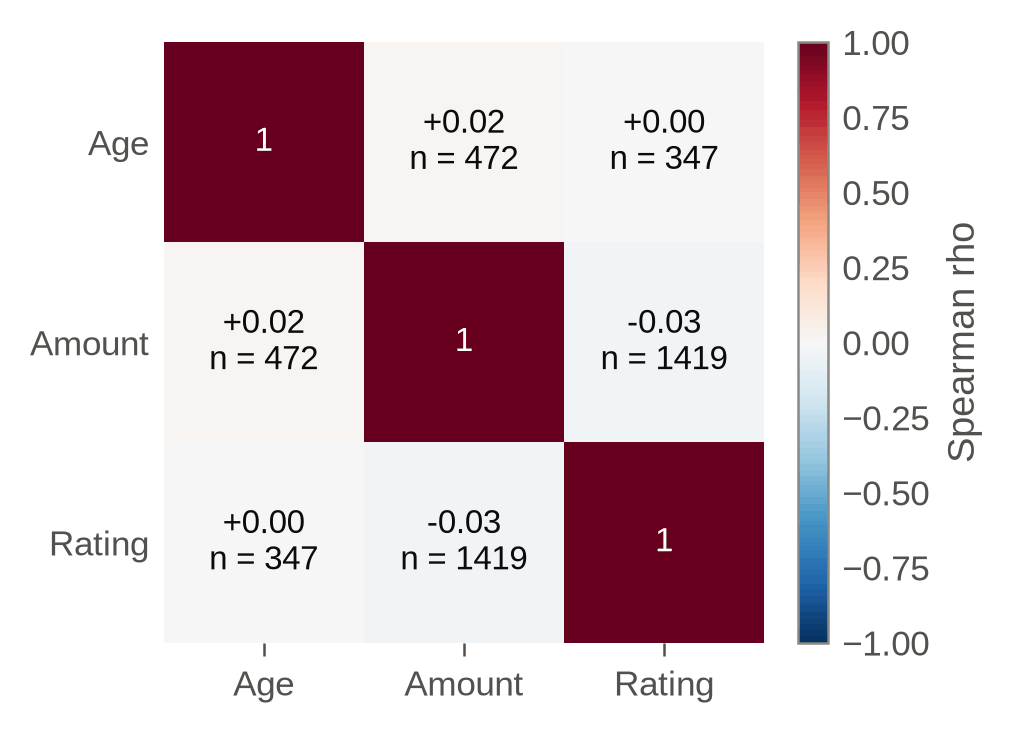
\includegraphics[width=0.62\linewidth]{08_correlations.png}
\caption{Spearman rank correlations between age, amount and rating, each on the
customers where both values are valid ($n$ in each cell). Every coefficient lies
between $-0.03$ and $+0.02$: none of the recorded attributes is associated with
spending.}
\end{figure}

% =====================================================================
\section{Statistical tests}

\begin{table}[H]\centering\singlespacing
\caption{Tests behind every segment statement of this report}
\small
\begin{tabular}{@{}llrrr@{}}
\toprule
\textbf{Question} & \textbf{Test} & \textbf{Statistic} & \textbf{$p$} & \textbf{$n$} \\ \midrule
Amount differs by category & Kruskal--Wallis $H$ & 3.72 & 0.445 & 1{,}464 \\
Amount differs, men against women & Mann--Whitney $U$ & 361{,}889 & 0.095 & 1{,}743 \\
Amount differs, Unknown against others & Mann--Whitney $U$ & 380{,}118 & 0.209 & 2{,}003 \\
Rating mix differs by category & $\chi^2$ (16 df) & 8.38 & 0.937 & 1{,}072 \\
Purchases differ across 32 months & $\chi^2$ (31 df) & 40.98 & 0.108 & 1{,}917 \\
Amount associated with rating & Spearman $\rho$ & $-0.03$ & 0.301 & 1{,}419 \\
Amount associated with age & Spearman $\rho$ & 0.02 & 0.702 & 472 \\
Amounts spread evenly & Kolmogorov--Smirnov $D$ & 0.019 & 0.488 & 2{,}003 \\
\bottomrule
\end{tabular}
\end{table}

None of the eight tests is significant at the 5\% level. This is itself the result:
the register does not separate customers who spend more from those who spend less,
and the monthly profile does not show a season. Uniform amounts, uniform ratings and
48 distinct names point to a synthetic or anonymised extract. The methods and the
pipeline transfer unchanged to real data; the business conclusions must be re-tested
on it.

% =====================================================================
\section{Insights and recommendations}

\subsection{Data capture is the first problem to solve}

Four of the six quality policies are breached: invalid dates (5.6\% against a 3\%
threshold), unknown category (26.9\% against 20\%), missing age (76.4\% against 30\%)
and missing rating (29.2\% against 25\%). The contact fields cannot reach a single
customer.

\textbf{Recommendation.} Enforce validation at entry: age between 1 and 100, a rating
widget limited to 1 to 5, a mandatory category, a calendar date picker, and unique,
verified contact details. Keep the automated quality gate in the publishing path
until the four policies pass. \emph{Owner: point-of-sale and CRM IT.}

\subsection{Revenue is \$1{,}021{,}324 on 2{,}003 recorded amounts}

The average ticket is \$509.90, the median \$519.42. 97 amounts are missing, so
revenue is a recorded total, not a complete one.

\textbf{Recommendation.} Publish revenue with its base and make the amount mandatory
for closed transactions. \emph{Owner: finance.}

\subsection{The Unknown category is the largest ``category''}

565 purchases have no category, more than Clothing or Electronics (323 each). Their
amounts do not differ from the others, so the known mix is a fair guide, but each
category total is understated by about a quarter.

\textbf{Recommendation.} Make the category mandatory at the point of sale before any
assortment decision. The 14\% revenue gap between Clothing and Toys comes from volume,
not from the ticket ($p = 0.45$). \emph{Owner: merchandising.}

\subsection{No customer attribute predicts spending}

Amounts do not differ by gender, category, age or rating, and are spread evenly
between \$5 and \$1{,}000.

\textbf{Recommendation.} Do not target campaigns on age, gender or category with
this data: none separates high from low spenders. Collect purchase history, channel
and basket content, the usual drivers of spend. \emph{Owner: marketing.}

\subsection{Satisfaction is mediocre and polarised}

The mean rating is 3.03 out of 5. 38.7\% of valid ratings are 1 or 2, in every
category alike.

\textbf{Recommendation.} Contact customers who rate 1 or 2 within a week, and add a
reason code to the rating to find the cause. \emph{Owner: customer service.}

\subsection{The monthly profile shows no seasonality}

The dip of August and September in the pooled chart is a coverage effect. On the true
monthly series, purchases are even ($p = 0.11$).

\textbf{Recommendation.} Do not plan stock or staff on the pooled chart. Report
purchases per calendar month, and re-test seasonality once three full years are
available. \emph{Owner: operations.}

% =====================================================================
\section{The interactive dashboard}

\F{dashboard.html} is a single self-contained file built with Plotly: open it in a
modern browser (Chrome or Edge, then Ctrl+F5), with no server and no installation.
The left navigation bar opens nine views: Dashboard, Data Explorer, Live Data,
Customers, Products, Trends, Data Quality, Insights and KPI Code. Filters on category,
gender, age band and rating update every key indicator, chart and table at once. The
header carries a live clock, an auto-refresh selector and the data-quality status;
the side panel offers dark and light themes, six accent colours and four fonts. The
Data Explorer exports the filtered table to CSV or Excel.

The dashboard is reproduced here without any modification. The captures were taken
with every filter cleared, at 1{,}920 by 1{,}057 pixels.

\subsection{Reading the dashboard against this report}

Every headline tile of the dashboard equals the report value: 2{,}100 customers,
\$1{,}021{,}324 revenue, \$510 average ticket, 3.03 mean rating, 54.4 mean age,
50 duplicates removed and 118 invalid dates. Four elements use a different base or
rule; they are listed so that no reader meets an unexplained difference.

\begin{table}[H]\centering\singlespacing
\caption{Reconciliation between dashboard elements and report indicators}
\small
\begin{tabularx}{\linewidth}{@{}p{4.6cm}X@{}}
\toprule
\textbf{Dashboard element} & \textbf{Base used and report equivalent} \\ \midrule
\emph{Gender mix} donut & All 2{,}100 customers: Male 44.9\%, Female 42.4\%,
Unknown 12.7\%. Report equivalent: 51.4\% / 48.6\% of the 1{,}833 known genders. \\
\emph{Purchases over time}, \emph{Monthly purchase trend}, \emph{Dynamic analytics} &
Three years pooled by month name. August and September count two years, the other
months three. Report equivalent: Figure~5 and Table~\ref{tab:pooled}. \\
\emph{Avg purchase by category} (Products) & Revenue divided by all customers of the
category, including the 97 without an amount (Clothing \$507). Report equivalent:
mean of recorded amounts (Clothing \$537). \\
\emph{Data quality control} alerts & One high, two medium and one low alert: Unknown
category graded medium, rating sparsity low. Pipeline policy
(\F{results/quality_alerts.json}): two high, two medium. Both give the status
ALERT. \\
\bottomrule
\end{tabularx}
\end{table}

The Data Explorer and Customers tables show the purchase date as captured, so the
118 flagged rows display 32/13/2020; they are excluded from every time-based chart.

\subsection{Dashboard}

\capture{01_dashboard_hero_kpis.png}{Dashboard, header and executive overview: live
clock, priorities, the six key indicators (customers, revenue, average ticket, rating,
age, data-quality status), KPI definitions, filters, purchases over time and gender
mix.}
\capture{02_dashboard_charts_top.png}{Dashboard, category volume, revenue by category,
age bands (the 1{,}605 customers without a valid age shown as \emph{Unknown}), rating
distribution and key insights.}
\capture{03_dashboard_category_age.png}{Dashboard, dynamic analytics (bars, lines or
area; revenue, volume or average ticket by month), live category pulse and the rolling
window of the clean-data stream.}
\capture{04_dashboard_rating_insights.png}{Dashboard, interactive category treemap (a
click filters every view), revenue against volume by category with the mean rating as
colour, and the live KPI pulse.}
\capture{16_dashboard_light_theme.png}{Dashboard in the light theme.}

\subsection{Data Explorer and Live Data}

\capture{08_explorer_top.png}{Data Explorer: search, gender and category filters,
CSV and Excel export, paginated over the 2{,}100 customers.}
\capture{09_live_data_top.png}{Live Data: the clean register streamed row by row,
with the live category mix, the rolling purchase amount and the quality flags of each
row.}

\subsection{Customers and Products}

\capture{10_customers_top.png}{Customers: one row per customer with age, gender,
category, amount, date and rating.}
\capture{11_products_top.png}{Products: customers, revenue, average purchase and mean
rating by category.}

\subsection{Trends}

\capture{12_trends_top.png}{Trends: monthly purchase trend (pooled by month name),
purchase amount distribution and rating mix.}

\subsection{Data Quality}

\capture{13_quality_top.png}{Data Quality: the four actionable alerts with their
recommendations, the defect counts (2{,}100 clean customers, 50 duplicates removed,
118 invalid dates, 5 categories) and the cleaning rules applied.}

\subsection{Insights and KPI Code}

\capture{14_insights_top.png}{Insights: the nine headline findings computed from the
clean register.}
\capture{15_kpi_code_top.png}{KPI Code: the exact pandas formula behind each indicator
(revenue and ticket, customers and mix, rating, data-quality rates), so that every
tile can be reproduced.}

% =====================================================================
\section{Pipeline and automated quality alerts}

The dashboard is only as reliable as the data it reads. The project therefore ships
the pipeline that produces and guards the clean register.

\begin{table}[H]\centering\singlespacing
\caption{Components of the pipeline}
\small
\begin{tabularx}{\linewidth}{@{}p{4.4cm}X@{}}
\toprule
\textbf{Component} & \textbf{Role} \\ \midrule
\F{etl/run_etl.py} & Extract the raw file, apply the cleaning rules, load
\F{data/customers_clean.csv}, write an audit (\F{results/etl_audit.json}). \\
\F{api/run_quality_alerts.py} & Compare the clean table with the policy thresholds;
exit code 0 (OK), 1 (WARN) or 2 (ALERT). \\
\F{api/notify_alerts.py} & Send the alerts to the console, a file, a webhook or
email (\F{api/notify_config.json}). \\
\F{api/metrics_server.py} & Expose the indicators and alerts to Prometheus. \\
\F{airflow/customer_analytics_etl_dag.py} & Run daily: ETL, then the quality gate,
then publication; an ALERT stops publication. \\
\F{grafana/}, \F{docker-compose.yml} & Prometheus and Grafana monitoring of the
indicators and alerts. \\
\bottomrule
\end{tabularx}
\end{table}

\begin{table}[H]\centering\singlespacing
\caption{Quality policies applied by the pipeline to the clean register}
\small
\begin{tabular}{@{}lrrlc@{}}
\toprule
\textbf{Policy} & \textbf{Value} & \textbf{Threshold} & \textbf{Severity} & \textbf{Breached} \\ \midrule
Invalid purchase dates & 5.62\% & 3\% & high & yes \\
Unknown product category & 26.90\% & 20\% & high & yes \\
Missing purchase amount & 4.62\% & 5\% & high & no \\
Missing age after purge & 76.43\% & 30\% & medium & yes \\
Missing or invalid rating & 29.19\% & 25\% & medium & yes \\
Duplicate CustomerID & 0 & 1 & medium & no \\
\bottomrule
\end{tabular}
\end{table}

The status is \textbf{ALERT}: two high-severity policies are breached. The duplicate
policy reads 0 because it is evaluated on the clean table, after the 50 duplicates
were removed; the ETL audit records the 50 removals. Missing amounts sit just below
their threshold and should be watched weekly.

% =====================================================================
\section{Limitations}

\textbf{One purchase per customer.} No repeat-purchase, retention or lifetime-value
indicator can be computed.

\textbf{Age rests on 495 customers}, 23.6\% of the file, and nothing shows that they
represent the others. Age bands are descriptive only.

\textbf{Ratings rest on 1{,}487 customers}, 70.8\% of the file. The 291 values of 10
may hide real scores typed on another scale.

\textbf{The extract looks synthetic.} 48 distinct names, two phone numbers, 144 emails,
and amounts and ratings spread evenly. Methods and pipeline transfer to real data;
the business conclusions must be re-tested on it.

\textbf{Association, not causation.} The absence of a relationship between spend and
the attributes recorded does not exclude drivers that are not recorded.

% =====================================================================
\section{Reproducibility}

Every number, table and figure of this report is produced by the notebook
\F{Customer-Analytics.ipynb} from the raw file \F{data/customers_raw.csv}. The
notebook writes the clean register (\F{data/customers_clean.csv}), the result tables
(\F{results/}) and the figures (\F{figures/}, PNG at 300~dpi), and checks that its
cleaning matches the production ETL. Once the capture is repaired at source,
re-running the notebook and the pipeline unchanged recomputes every flag, indicator,
test, figure and alert.

\vspace{0.3cm}
\noindent\hfill\begin{minipage}{7cm}\begin{flushright}\singlespacing
\textbf{KOUAME Koffi Fid\`ele}\\
Data Analysis Internship\\
\href{mailto:koffifidelek59@gmail.com}{koffifidelek59@gmail.com}
\end{flushright}\end{minipage}

\end{document}
